\documentclass[UTF8]{ctexart}
\usepackage{ctex}
\usepackage{geometry}
\usepackage{enumitem}
\usepackage{indentfirst}
\usepackage{color}
\usepackage{fancyhdr}
\usepackage{amsmath}
\usepackage{graphicx}
\usepackage{amssymb}
\usepackage{tikz}
\usepackage{cases}
\usepackage{array}
\usepackage{pgfplots}
\usepackage{tkz-euclide}
\usepackage{mathrsfs}
% 设置纸张和页边距——A4
\geometry{papersize={21cm,29.7cm}}
\geometry{left=3.18cm,right=3.18cm,top=2.54cm,bottom=2.54cm}

% 一级标题靠左
\CTEXsetup[format={\Large\bfseries}]{section}

% 去除页眉
\pagestyle{plain}

%设置段间距
\addtolength{\parskip}{.4em}
%%设置行间距
%\usepackage{setspace}
%\setstretch{2.5}

% 开始文档内容
\begin{document}

\title{信号与系统课程笔记:Lecture 16 \\
理想低通滤波器(Ideal Lowpass Filter)}
\author{授课教师:秦雨潇 \\
        笔记记录:曹时成}
\date{2023 年 11 月 8 日(第十周,周三)}
\maketitle

\section{复习}
$e^{j\omega_0 t}\longrightarrow $ \boxed{H(\omega)} $\longrightarrow H(\omega_0 )e^{j\omega_0t}$ \qquad 输出的频率和振幅取决于输入的 $\omega_0$ \par
根据 LTI 系统: \par
$f(t)\ast h(t)=y(t)\Leftarrow \delta (t)\ast h(t)=h(t)$ \par
$\frac{1}{2\pi}\int_{\mathbb{R}} F(\omega)e^{j\omega t} d\omega\Longleftrightarrow \frac{1}{2\pi}\int_{\mathbb{R}} F(\omega)H(\omega)e^{j\omega t} d\omega$\par
$y(t)=\mathscr{F}^{-1}\{F(\omega)H(\omega)\}$ \par
结论:$H(\omega)$反应了$y(t)$输出的幅度和初始相位的变化。 \par
\section{$H(\omega)$}
$H(\omega)$: 频率响应函数(Frequency Response Function/转移函数(Transformation Function) \par
$ h(t)$:“冲激响应”(Impulse Response Function, IRF)\par
Question:How to get $H(\omega)$ ?\par
(1) $H(\omega)=\mathscr{F}^{-1}\{h(t)\}$\par
(2) $F(\omega)H(\omega)=Y(\omega)\implies H(\omega)=\frac{Y(\omega)}{F(\omega)}  $\par
(3) 定义:$H(\omega)=| H(\omega)\vert e^{j\angle H(\omega)}$   \par
$| H(\omega)\vert$为频幅响应,$e^{j\angle H(\omega)}$为相频响应。\par
\subsection{例 1: ODE $\rightarrow $ linear}
题:$y'(t)+2y(t)=f(t)$,$f(t)=e^{-t}u(t)$,求$y(t)$ \par
解:根据时域微分性质 $f^n(t)=(jw)^nF(w)$ \par
\qquad $(jw+2)Y(w)=f(w)$ \par
\qquad $H(w)=\frac{Y(\omega)}{F(\omega)}=(jw+2)$ \par
\qquad $Y(\omega)=H(\omega)F(\omega)=\frac{1}{jw+2} \frac{1}{jw+1}=\frac{1}{jw+1}-\frac{1}{jw+2}$ \par
\qquad 故:$y(t)=e^{-t}u(t)-e^{-2t}u(t)$ \par
\subsection{例 2: PDE $\rightarrow $ODE $\rightarrow $ linear}
题:傅里叶热传导方程求解  $\frac{\partial u(x,t)}{\partial t}=\alpha ^2\frac{\partial^2 u(x,t)}{\partial x^2} $ \par
解:\par
\qquad 令:$\mathscr{F}\{u(x,t)\}=\hat{u}(w,t) $\par
\qquad 根据时域微分性质有:$\alpha ^2\frac{\partial^2 (x,t)}{\partial x^2}=(jw)^2 \hat{u}(w,t)= -\alpha ^2w^2\hat{u}(w,t)$\par
\qquad 此外:$\mathscr{F}\{\frac{\partial u(x,t)}{\partial t}\}=\frac{\partial }{\partial t}\hat{u}(w,t)$\par
\qquad 令:$y(t)=\hat{u}(w,t)\hat{u}(w,0) $ 其中:$\hat{u}(w,t)=e^{-\alpha ^2w^2t}\hat{u}(w,0) $\par
\qquad 有:$y'(t)=-\alpha ^2w^2y(t) $\par
\qquad \qquad  $y(t)=e^{-\alpha ^2w^2t}$\par
\qquad \qquad $y(t)=\hat{u}(w,t)=\mathscr{F}\{u(x,t)\}=e^{-\alpha ^2w^2t}$ 是正态分布函数\par
由于正态分布函数的傅里叶变换也是正态分布函数且 $\hat{u}(w,t)=e^{-\alpha ^2w^2t}\hat{u}(w,0) $\par
\qquad 故:$u(x,t)=\mathscr{F}^{-1}\{y(t)\}\ast u(x,0) $\par
\section{无失真传输}
\subsection{无失真系统}
定义:输入和输出相比,只有幅度大小和出现时间的先后不同这两种“变化”,而没有波形的变化。\par

\begin{figure}[h]
    \centering         %使图片居中放置
    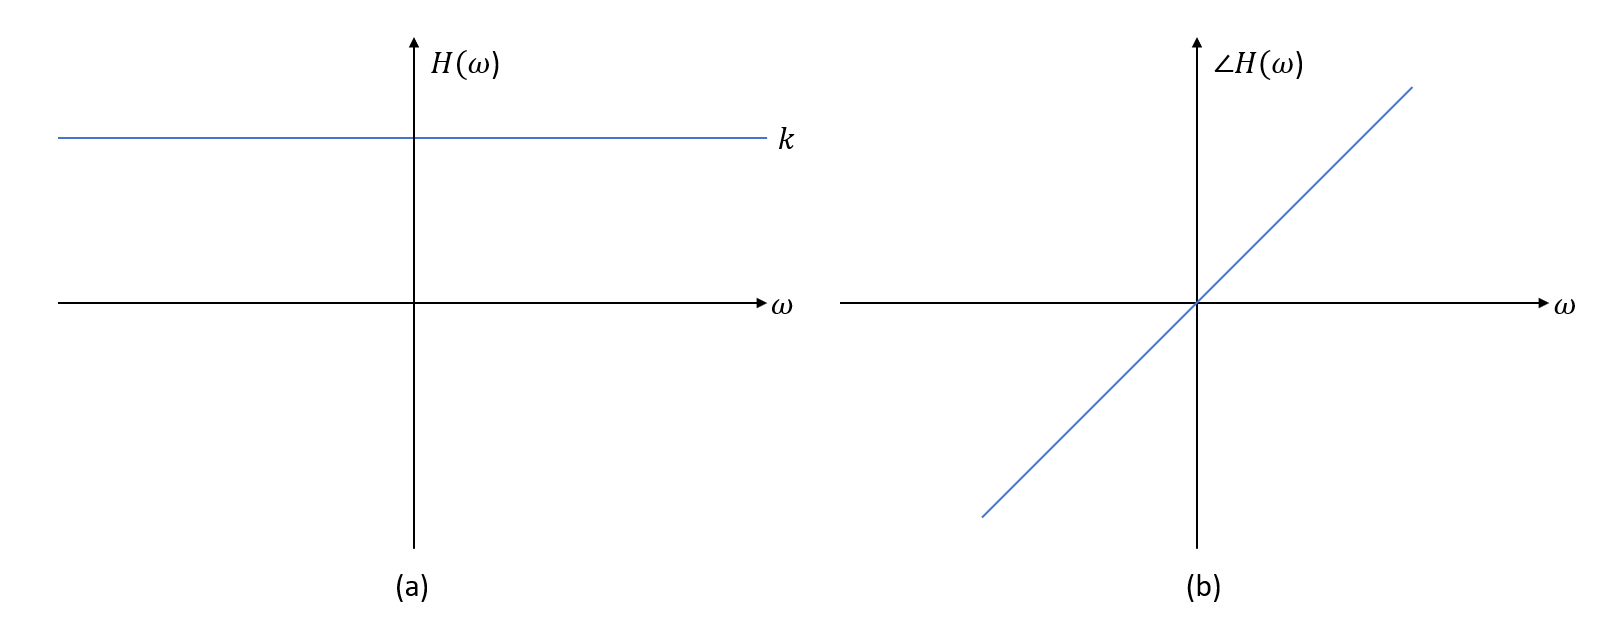
\includegraphics[scale=0.4]{1.png}
    \caption{无失真传输系统在频域的表示。(a)幅频;(b)相频。}
\end{figure} \par
\,\par
数学表示:\par
$f(t)\longrightarrow kf(t-t_d)$,根据时移性质有:\par
$F(w)\longrightarrow kF(w)e^{-jwt_d}$\par
$ H(\omega)=\frac{Y(\omega)}{F(\omega)} =ke^{-jwt_d} \equiv $无失真传输系统\par
结论1:无失真系统在物理层面不存在
\subsection{理想低通滤波器(Ideal Lowpass Filter (LPF)}
无失真系统 \(\xrightarrow{\text{退而求其次}}\) Ideal LPF \par
定义:在“有限带宽”$[-w_c,w_c] $范围内,幅频是常数,相频是线性即可。
\begin{figure}[h]
    \centering         %使图片居中放置
    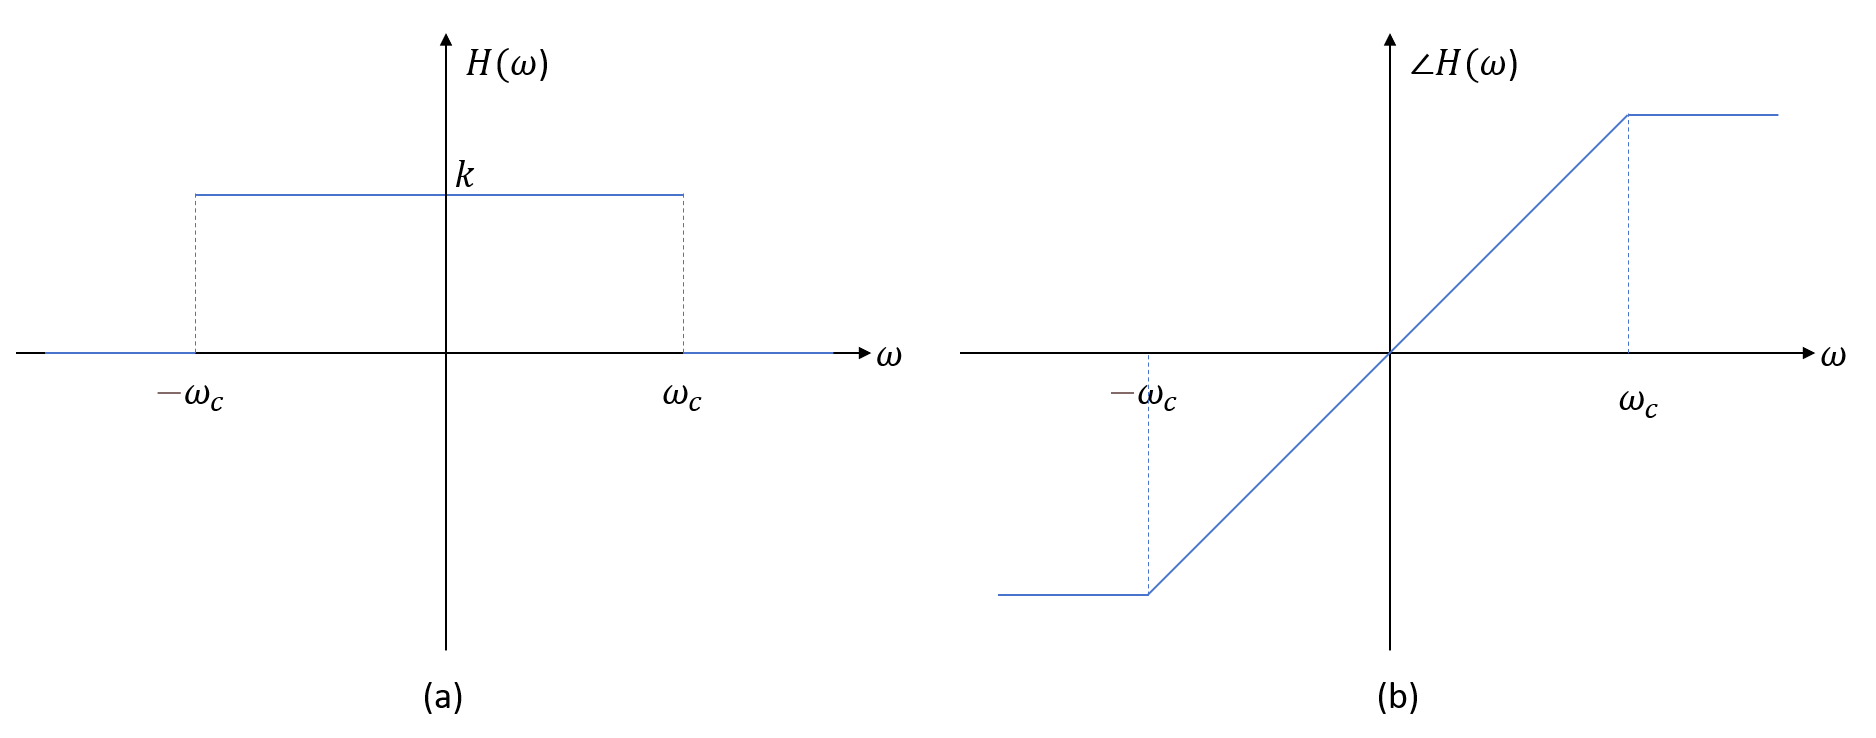
\includegraphics[scale=0.32]{2.png}
    \caption{理想低通滤波器在频域的表示。(a)幅频;(b)相频。}
\end{figure}
$w_c$为截止频率(cut-off frequency),一般$w_c$的值为信号第一次衰减为0时对应的频率或者信号衰减为3dB时对应的频率。\par
结论2:Ideal LPF 也不存在
\subsection{例题}
对于一个信号$f(t)$通过下图所示的 Ideal LPF,信号是否失真?\par
\begin{figure}[h]
    \centering         %使图片居中放置
    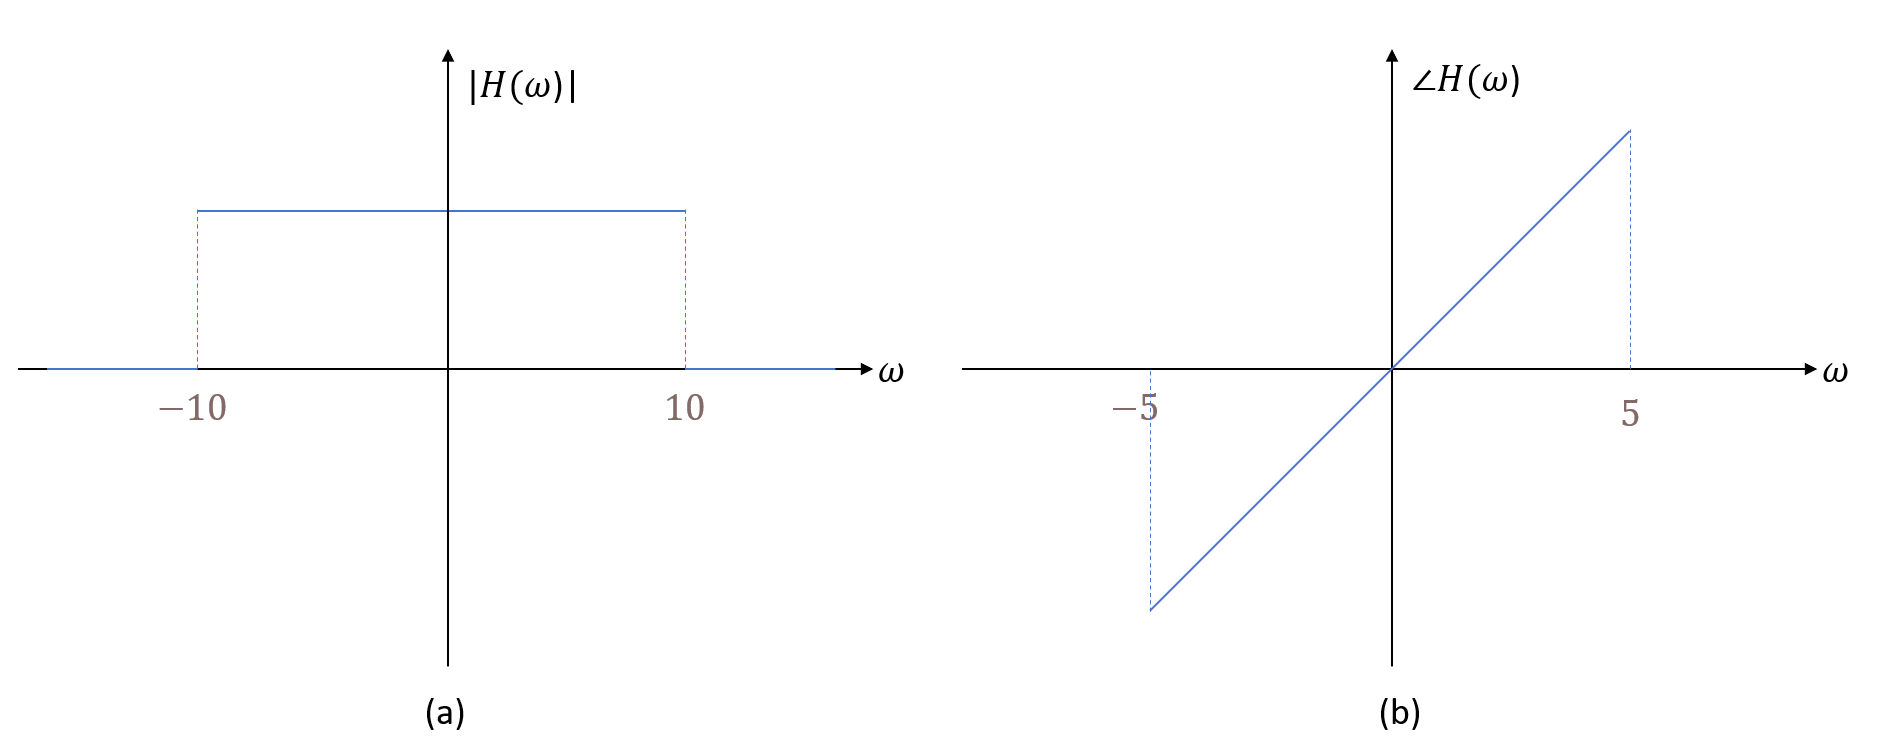
\includegraphics[scale=0.22]{3.png}
    \caption{一个理想低通滤波器在频域的表示。(a)幅频;(b)相频。}
\end{figure}
(1)$f(t)=cost+cos8t$ \qquad \qquad \quad 失真 \par
(2)$f(t)=sin2t+sin4t$ \qquad \qquad \; 无失真 \par
(3)$f(t)=sin2t sin4t$ \qquad \qquad \qquad 失真 \par
(4)$f(t)=cos^24t$  $\Rightarrow 1+2cos8t$ \qquad 失真\par
\subsection{卷积只能算零状态响应}
对于$H(\omega)F(\omega)=Y(\omega)\Leftrightarrow f(t)\ast h(t)=y(t)$来说,卷积算的是零状态响应。
\end{document}